\documentclass[11pt,a4paper,]{article}
\usepackage{lmodern}

\usepackage{amssymb,amsmath}
\usepackage{ifxetex,ifluatex}
\usepackage{fixltx2e} % provides \textsubscript
\ifnum 0\ifxetex 1\fi\ifluatex 1\fi=0 % if pdftex
  \usepackage[T1]{fontenc}
  \usepackage[utf8]{inputenc}
\else % if luatex or xelatex
  \usepackage{unicode-math}
  \defaultfontfeatures{Ligatures=TeX,Scale=MatchLowercase}
\fi
% use upquote if available, for straight quotes in verbatim environments
\IfFileExists{upquote.sty}{\usepackage{upquote}}{}
% use microtype if available
\IfFileExists{microtype.sty}{%
\usepackage[]{microtype}
\UseMicrotypeSet[protrusion]{basicmath} % disable protrusion for tt fonts
}{}
\PassOptionsToPackage{hyphens}{url} % url is loaded by hyperref
\usepackage[unicode=true]{hyperref}
\hypersetup{
            pdftitle={How will the stock market react to the PCA: Envidence From Yahoo Finance Stock Market},
            pdfborder={0 0 0},
            breaklinks=true}
\urlstyle{same}  % don't use monospace font for urls
\usepackage{geometry}
\geometry{a4paper, centering, text={16cm,24cm}}
\usepackage[style=apa,]{biblatex}
\addbibresource{references.bib}
\usepackage{longtable,booktabs}
% Fix footnotes in tables (requires footnote package)
\IfFileExists{footnote.sty}{\usepackage{footnote}\makesavenoteenv{long table}}{}
\usepackage{graphicx,grffile}
\makeatletter
\def\maxwidth{\ifdim\Gin@nat@width>\linewidth\linewidth\else\Gin@nat@width\fi}
\def\maxheight{\ifdim\Gin@nat@height>\textheight\textheight\else\Gin@nat@height\fi}
\makeatother
% Scale images if necessary, so that they will not overflow the page
% margins by default, and it is still possible to overwrite the defaults
% using explicit options in \includegraphics[width, height, ...]{}
\setkeys{Gin}{width=\maxwidth,height=\maxheight,keepaspectratio}
\IfFileExists{parskip.sty}{%
\usepackage{parskip}
}{% else
\setlength{\parindent}{0pt}
\setlength{\parskip}{6pt plus 2pt minus 1pt}
}
\setlength{\emergencystretch}{3em}  % prevent overfull lines
\providecommand{\tightlist}{%
  \setlength{\itemsep}{0pt}\setlength{\parskip}{0pt}}
\setcounter{secnumdepth}{5}

% set default figure placement to htbp
\makeatletter
\def\fps@figure{htbp}
\makeatother


\title{How will the stock market react to the PCA: Envidence From Yahoo Finance Stock Market}

%% MONASH STUFF

%% CAPTIONS
\RequirePackage{caption}
\DeclareCaptionStyle{italic}[justification=centering]
 {labelfont={bf},textfont={it},labelsep=colon}
\captionsetup[figure]{style=italic,format=hang,singlelinecheck=true}
\captionsetup[table]{style=italic,format=hang,singlelinecheck=true}


%% FONT
\RequirePackage{bera}
\RequirePackage[charter,expert,sfscaled]{mathdesign}
\RequirePackage{fontawesome}

%% HEADERS AND FOOTERS
\RequirePackage{fancyhdr}
\pagestyle{fancy}
\rfoot{\Large\sffamily\raisebox{-0.1cm}{\textbf{\thepage}}}
\makeatletter
\lhead{\textsf{\expandafter{\@title}}}
\makeatother
\rhead{}
\cfoot{}
\setlength{\headheight}{15pt}
\renewcommand{\headrulewidth}{0.4pt}
\renewcommand{\footrulewidth}{0.4pt}
\fancypagestyle{plain}{%
\fancyhf{} % clear all header and footer fields
\fancyfoot[C]{\sffamily\thepage} % except the center
\renewcommand{\headrulewidth}{0pt}
\renewcommand{\footrulewidth}{0pt}}

%% MATHS
\RequirePackage{bm,amsmath}
\allowdisplaybreaks

%% GRAPHICS
\RequirePackage{graphicx}
\setcounter{topnumber}{2}
\setcounter{bottomnumber}{2}
\setcounter{totalnumber}{4}
\renewcommand{\topfraction}{0.85}
\renewcommand{\bottomfraction}{0.85}
\renewcommand{\textfraction}{0.15}
\renewcommand{\floatpagefraction}{0.8}


%\RequirePackage[section]{placeins}

%% SECTION TITLES


%% SECTION TITLES
\RequirePackage[compact,sf,bf]{titlesec}
\titleformat*{\section}{\Large\sf\bfseries\color[rgb]{0.7,0,0}}
\titleformat*{\subsection}{\large\sf\bfseries\color[rgb]{0.7,0,0}}
\titleformat*{\subsubsection}{\sf\bfseries\color[rgb]{0.7,0,0}}
\titlespacing{\section}{0pt}{2ex}{.5ex}
\titlespacing{\subsection}{0pt}{1.5ex}{0ex}
\titlespacing{\subsubsection}{0pt}{.5ex}{0ex}


%% TITLE PAGE
\def\Date{\number\day}
\def\Month{\ifcase\month\or
 January\or February\or March\or April\or May\or June\or
 July\or August\or September\or October\or November\or December\fi}
\def\Year{\number\year}

%% LINE AND PAGE BREAKING
\sloppy
\clubpenalty = 10000
\widowpenalty = 10000
\brokenpenalty = 10000
\RequirePackage{microtype}

%% PARAGRAPH BREAKS
\setlength{\parskip}{1.4ex}
\setlength{\parindent}{0em}

%% HYPERLINKS
\RequirePackage{xcolor} % Needed for links
\definecolor{darkblue}{rgb}{0,0,.6}
\RequirePackage{url}

\makeatletter
\@ifpackageloaded{hyperref}{}{\RequirePackage{hyperref}}
\makeatother
\hypersetup{
     citecolor=0 0 0,
     breaklinks=true,
     bookmarksopen=true,
     bookmarksnumbered=true,
     linkcolor=darkblue,
     urlcolor=blue,
     citecolor=darkblue,
     colorlinks=true}

\usepackage[showonlyrefs]{mathtools}
\usepackage[no-weekday]{eukdate}

%% BIBLIOGRAPHY

\makeatletter
\@ifpackageloaded{biblatex}{}{\usepackage[style=authoryear-comp, backend=biber, natbib=true]{biblatex}}
\makeatother
\ExecuteBibliographyOptions{bibencoding=utf8,minnames=1,maxnames=3, maxbibnames=99,dashed=false,terseinits=true,giveninits=true,uniquename=false,uniquelist=false,doi=false, isbn=false,url=true,sortcites=false}

\DeclareFieldFormat{url}{\texttt{\url{#1}}}
\DeclareFieldFormat[article]{pages}{#1}
\DeclareFieldFormat[inproceedings]{pages}{\lowercase{pp.}#1}
\DeclareFieldFormat[incollection]{pages}{\lowercase{pp.}#1}
\DeclareFieldFormat[article]{volume}{\mkbibbold{#1}}
\DeclareFieldFormat[article]{number}{\mkbibparens{#1}}
\DeclareFieldFormat[article]{title}{\MakeCapital{#1}}
\DeclareFieldFormat[article]{url}{}
%\DeclareFieldFormat[book]{url}{}
%\DeclareFieldFormat[inbook]{url}{}
%\DeclareFieldFormat[incollection]{url}{}
%\DeclareFieldFormat[inproceedings]{url}{}
\DeclareFieldFormat[inproceedings]{title}{#1}
\DeclareFieldFormat{shorthandwidth}{#1}
%\DeclareFieldFormat{extrayear}{}
% No dot before number of articles
\usepackage{xpatch}
\xpatchbibmacro{volume+number+eid}{\setunit*{\adddot}}{}{}{}
% Remove In: for an article.
\renewbibmacro{in:}{%
  \ifentrytype{article}{}{%
  \printtext{\bibstring{in}\intitlepunct}}}

\AtEveryBibitem{\clearfield{month}}
\AtEveryCitekey{\clearfield{month}}

\makeatletter
\DeclareDelimFormat[cbx@textcite]{nameyeardelim}{\addspace}
\makeatother

\author{\sf\Large\textbf{ Kaiwen Jin}\\ {\sf\large 26686953\\[0.5cm]} \sf\Large\textbf{ Zhiruo Zhang}\\ {\sf\large 28009487\\[0.5cm]} \sf\Large\textbf{ Jinhao Luo}\\ {\sf\large 29012449\\[0.5cm]}}

\date{\sf\Date~\Month~\Year}
\makeatletter
\lfoot{\sf Jin, Zhang, Luo: \@date}
\makeatother


%%%% PAGE STYLE FOR FRONT PAGE OF REPORTS

\makeatletter
\def\organization#1{\gdef\@organization{#1}}
\def\telephone#1{\gdef\@telephone{#1}}
\def\email#1{\gdef\@email{#1}}
\makeatother
  \organization{ETF5500 Assignment2}

  \def\name{Department of\newline Econometrics \&\newline Business Statistics}

  \telephone{(03) 9905 2478}

  \email{BusEco-Econometrics@monash.edu}

\def\webaddress{\url{http://buseco.monash.edu/ebs/consulting/}}
\def\abn{12 377 614 012}
\def\logo{
\includegraphics[width=6cm]{MBSportrait}}
\def\extraspace{\vspace*{1.6cm}}
\makeatletter
\def\contactdetails{\faicon{phone} & \@telephone \\
                    \faicon{envelope} & \@email}
\makeatother

%%%% FRONT PAGE OF REPORTS

\def\reporttype{Report for}

\long\def\front#1#2#3{
\newpage
\begin{singlespacing}
\thispagestyle{empty}
\vspace*{-1.4cm}
\hspace*{-1.4cm}
\hbox to 16cm{
  \hbox to 6.5cm{\vbox to 14cm{\vbox to 25cm{
    \logo
    \vfill
    \parbox{6.3cm}{\raggedright
      \sf\color[rgb]{0.00,0.00,0.70}
      {\large\textbf{\name}}\par
      \vspace{.7cm}
      \tabcolsep=0.12cm\sf\small
      \begin{tabular}{@{}ll@{}}\contactdetails
      \end{tabular}
      \vspace*{0.3cm}\par
      ABN: \abn\par
    }
  }\vss}\hss}
  \hspace*{0.2cm}
  \hbox to 1cm{\vbox to 14cm{\rule{1pt}{26.8cm}\vss}\hss\hfill}
  \hbox to 10cm{\vbox to 14cm{\vbox to 25cm{
      \vspace*{3cm}\sf\raggedright
      \parbox{11cm}{\sf\raggedright\baselineskip=1.2cm
         \fontsize{24.88}{30}\color[rgb]{0.70,0.00,0.00}\sf\textbf{#1}}
      \par
      \vfill
      \large
      \vbox{\parskip=0.8cm #2}\par
      \vspace*{2cm}\par
      \reporttype\\[0.3cm]
      \hbox{#3}%\\[2cm]\
      \vspace*{1cm}
      {\large\sf\textbf{\Date~\Month~\Year}}
   }\vss}
  }}
\end{singlespacing}
\newpage
}

\makeatletter
\def\titlepage{\front{\expandafter{\@title}}{\@author}{\@organization}}
\makeatother

\usepackage{setspace}
\setstretch{1.5}

%% Any special functions or other packages can be loaded here.
\usepackage{booktabs}
\usepackage{longtable}
\usepackage{array}
\usepackage{multirow}
\usepackage{wrapfig}
\usepackage{float}
\usepackage{colortbl}
\usepackage{pdflscape}
\usepackage{tabu}
\usepackage{threeparttable}
\usepackage{threeparttablex}
\usepackage[normalem]{ulem}
\usepackage{makecell}
\usepackage{xcolor}


\begin{document}
\titlepage

{
\setcounter{tocdepth}{2}
\tableofcontents
}
\clearpage

\hypertarget{introduction}{%
\section{Introduction}\label{introduction}}

In the financial market, the value of stocks would be investigated by many different variables. However, a large number of stocks make investors hard to make their decision. Therefore, this report would apply linear combination (LC) by combining the variables into an index and utilise principal component analysis (PCA) to evaluate the performance of stocks.

Besides, this report will also consider the accuracy of PCA and will discuss the potential limitation of PCA in stocks performance evaluation. Based on the result, Clustering Analysis as a comparative approach will also be provided.

At last, some useful suggestions for the stocks choosing will be concluded, as well as concluding the biases generated from the analysis.

The appendix will contain some notes to improve the understanding of our reports.

\hypertarget{data-description}{%
\section{Data Description}\label{data-description}}

\hypertarget{description}{%
\subsection{Description}\label{description}}

Our data was sourced from \href{https://au.finance.yahoo.com/}{Yahoo Finance} and it contains 18 variables of 147 stocks from five major financial indices. Those 18 variables could be further classified into 3 categories. The first categories capture \textbf{Name}, \textbf{Symbol}, \textbf{Market}, \textbf{Sector}, \textbf{Industry} which are related to the background of those stocks. The second and third categories provide some measurement of the value and risk which are related to the stocks. The further description of those variables is shown in Table \ref{tab:variables-table}.

\begin{table}

\caption{\label{tab:variables-table}Information of variables of the original data}
\centering
\begin{tabular}[t]{l|l|>{\raggedright\arraybackslash}p{170px}}
\hline
Variable & Abbreviation & Description\\
\hline
Name & / & The full company name of each stock\\
\hline
Symbol & / & The abbreviation of each stock\\
\hline
Market & / & Major financial indices\\
\hline
Sector & / & The belonging section of a stock\\
\hline
Industry & / & The belonging industry of a stock\\
\hline
Market capitalization & intra\_day & How much a company is worth as determined by the stock market\\
\hline
Enterprise value & ent\_value & A measure of a company's total value\\
\hline
Trailing P/E & trail\_pe & Price to Earning Ratio based on the earnings per share over the previous 12 months\\
\hline
Forward P/E ratio & for\_pe & Estimate further earnings per share in the next 12 months\\
\hline
PEG ratio & peg & Enhances the P/E ratio by adding the expected earnings growth into calculation\\
\hline
P/S ratio & ttm & Price to Sales ratio, a valuation ratio by comparing a company’s stock price to its revenue\\
\hline
P/B ratio & mrq & Price to Book ratio is a measurement of the market's valuation of a company relative to its book value\\
\hline
Enterprise value-to-revenue & rev & Also refers as the EV/R, it measures the value of a stock that compares a company's enterprise value to its revenue\\
\hline
EV/EBITDA & ebitda & Enterprise value to earnings before interest, taxed, depreciation and amortization ratio compares the value of a company, debt included to the company's cash earnings less non-cash expenses\\
\hline
Total ESG risk score & tot\_risk & The overall rating scores based on the Morningstar Sustainability Rating systems\\
\hline
Environmental Risk Score & envir\_risk & Evaluation scores of the portfolios performance when they meet the environmental challenges\\
\hline
Social Risk Score & social\_risk & Evaluation scores of the portfolios performance when they meet the social challenges\\
\hline
Governance Risk Score & gover\_risk & Evaluation scores of the portfolios performance when they meet the governance challenges\\
\hline
\end{tabular}
\end{table}

\hypertarget{limitation}{%
\subsection{Limitation}\label{limitation}}

This part will provide us an introduction about the limitation of the dataset, and it is shown below:

\begin{itemize}
\tightlist
\item
  This dataset contains a lot of missing value which would cause some bias in our final result
\item
  This dataset does not contain enough observations. The insufficient sample space will make our final result become unreliable. Also, if we further filter out the missing values, the sample size of the data would be even smaller. And the relatively small sample would not be representative enough to clarify the overall condition.
\item
  There is some inconsistency between the total ESG risk score and the sum of individual risk score. This inconsistency would directly increase the error in our final output.
\end{itemize}

Those limitations would be further discussed in the following sections. At last, the biases of analysis which generate from the limitations would be concluded.

\hypertarget{analysis}{%
\section{Analysis}\label{analysis}}

\hypertarget{preliminary-analysis}{%
\subsection{Preliminary Analysis}\label{preliminary-analysis}}

We will tidy our original dataset by removing the missing variables and further figure out other features. Figure \ref{fig:vis-data} shows the general data structure and it could be classified into three types which are character, numeric and missing value.

\begin{figure}
\centering
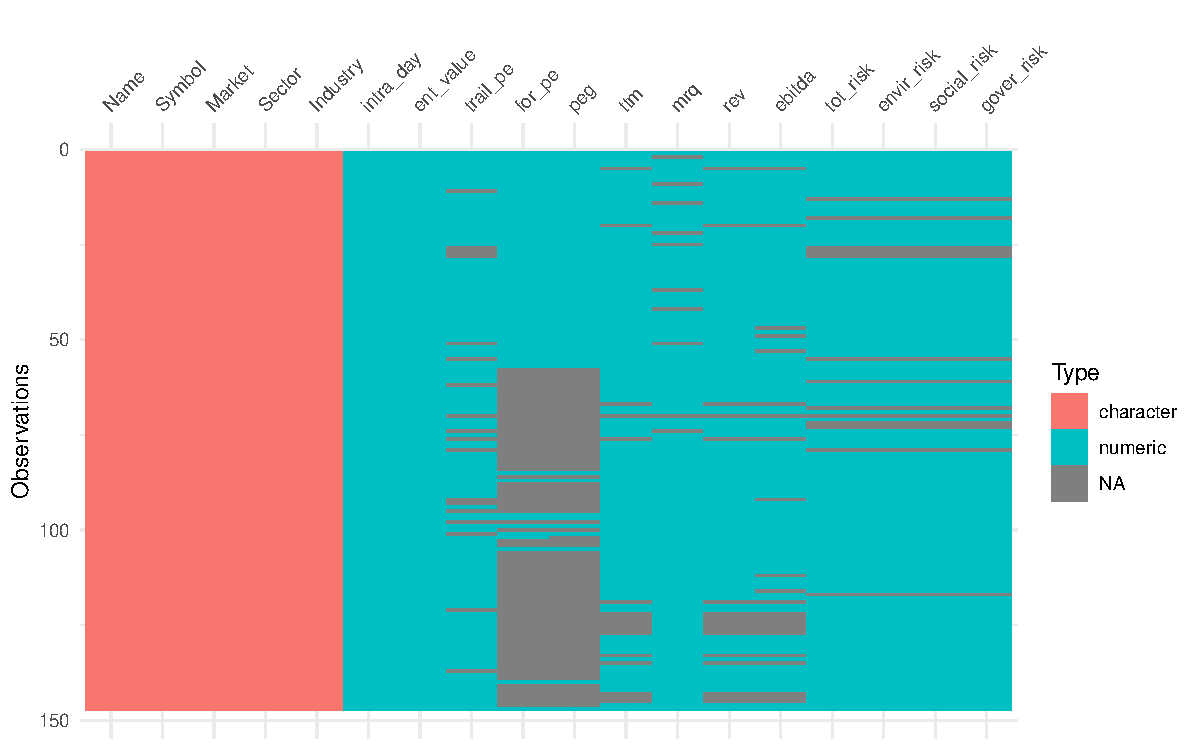
\includegraphics{ass2_files/figure-latex/vis-data-1.pdf}
\caption{\label{fig:vis-data}The data structure of original data}
\end{figure}

Table \ref{tab:summary-table} indicates that the initial 147 observations have up to 102 missing value and also some potential outliers.

\begin{table}

\caption{\label{tab:summary-table}Summary table of original data}
\centering
\begin{tabular}[t]{l|l|l|l|l|l}
\hline
Variable & Min & Median & Mean & Max & NA\\
\hline
intra\_day & -2 & 63 & 95065 & 5110000 & NA\\
\hline
ent\_value & -264 & 70 & 85683 & 5130000 & NA\\
\hline
trail\_pe & 0.48 & 20.11 & 43.62 & 1479.29 & 18\\
\hline
for\_pe & 3.59 & 19.92 & 43.04 & 1044.81 & 80\\
\hline
peg & -62.380 & 2.405 & 15.223 & 713.670 & 81\\
\hline
ttm & 0.9 & 2.8 & 9.941 & 548.150 & 17\\
\hline
mrq & 0.1 & 5.4 & 174.16 & 11765.96 & 10\\
\hline
rev & -27.720 & 2.875 & 9.827 & 5411.160 & 17\\
\hline
ebitda & -465.460 & 13.765 & 19.461 & 1117.510 & 23\\
\hline
tot\_risk & 11 & 23 & 25.39 & 75 & 13\\
\hline
envir\_risk & 0 & 4 & 6.731 & 62 & 13\\
\hline
social\_risk & 3 & 10 & 11.4 & 88 & 13\\
\hline
gover\_risk & 3 & 8 & 9.343 & 80 & 13\\
\hline
\end{tabular}
\end{table}

Most of the variables have a small median and mean, but an extremely high maximum value. Those extreme value would dominate our Principle Component Analysis and those outliers are shown in Table \ref{tab:outliers-table}.

\begin{table}

\caption{\label{tab:outliers-table}The summary table of outliers in each variables}
\centering
\begin{tabular}[t]{l|l}
\hline
variable & outlier\\
\hline
intra\_day & MSFT, AAPL\\
\hline
ent\_value & MSFT, AAPL\\
\hline
trail\_pe & TSLA\\
\hline
for\_pe & ILMN, TSLA\\
\hline
peg & DIS, VZ, KO, MMM, CVX, PCAR, CAT, XOM\\
\hline
ttm & ILMN, V\\
\hline
mrq & TSLA\\
\hline
rev & ILMN, V\\
\hline
ebitda & INTU, ILMN, TSLA, NKE\\
\hline
\end{tabular}
\end{table}

New dataset \textbf{stocks} will be generated by removing the missing value.

\hypertarget{principle-component-analysis}{%
\subsection{Principle Component Analysis}\label{principle-component-analysis}}

\hypertarget{value-analysis}{%
\subsubsection{Value Analysis}\label{value-analysis}}

Value analysis will be conducted by removing the high influential outliers. We also need to standardize the data due to the different units.

\begin{figure}
\centering
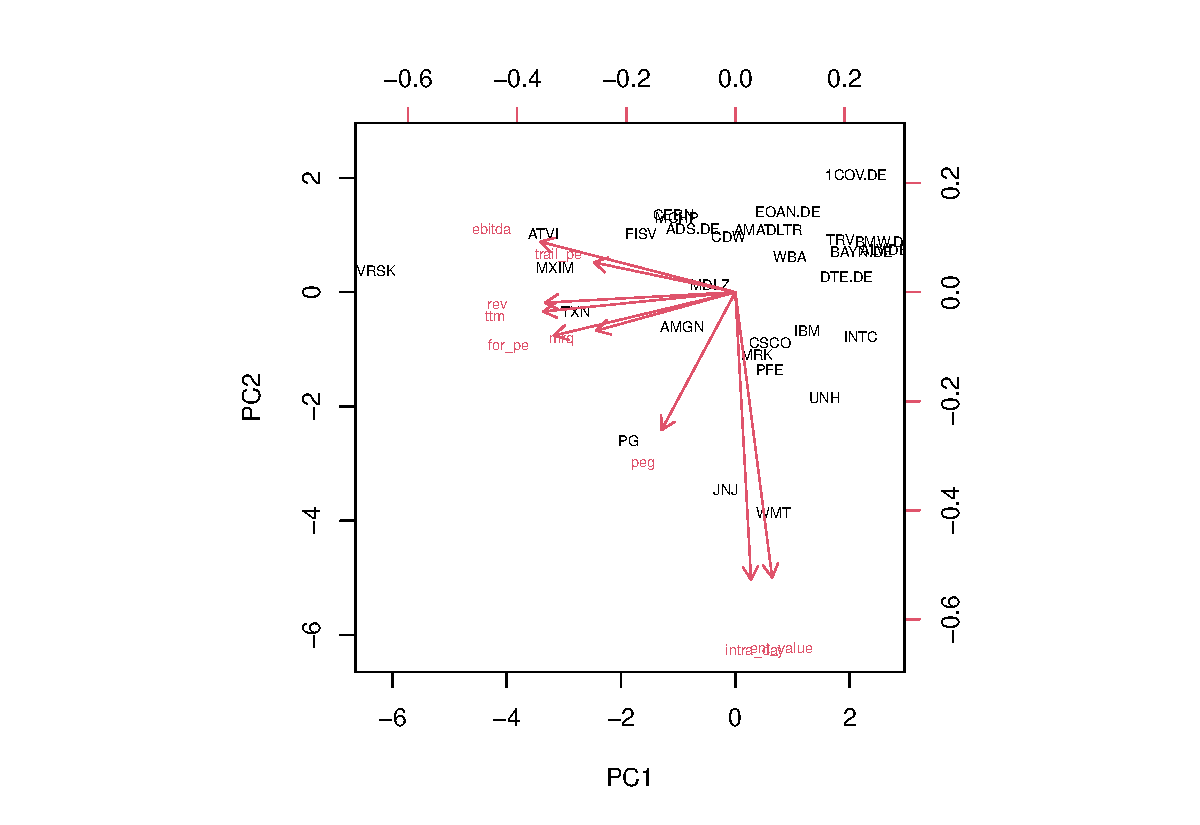
\includegraphics{ass2_files/figure-latex/pca-cor-1.pdf}
\caption{\label{fig:pca-cor}Correlation Biplot of PCA of stocks' value}
\end{figure}

Referring to the PCA value table, we could notice that PC1 is positive correlated with the measurement of company value which is \textbf{intra\_day} and \textbf{ent\_value}. PC2 is positive correlated with the stock earnings ratio (\textbf{ebitda} and \textbf{trail\_pe}) which means that the increase in the stock earnings ratio will increase PC2 slightly. We could notice that the variables which are related to the price-based evaluation of the stock are pretty close to the PC2.

Meanwhile, according to Figure \ref{fig:pca-cor} the narrow angle between \textbf{intra\_day} and \textbf{ent\_value} could highlight their strong association and the nearly 90 degree angle with \textbf{for\_eg},\textbf{ttm}, \textbf{mrq}, \textbf{rev} states the zero relationship. Furthermore, we could say that the angle between the measurement of company value and \textbf{ebita}, \textbf{trail\_pe} is close to 180 degree, their relationship should be negative. In other words, market value of a company will not influence its stock price and earn per share, but price and earnings will highly impact each other.

\begin{figure}
\centering
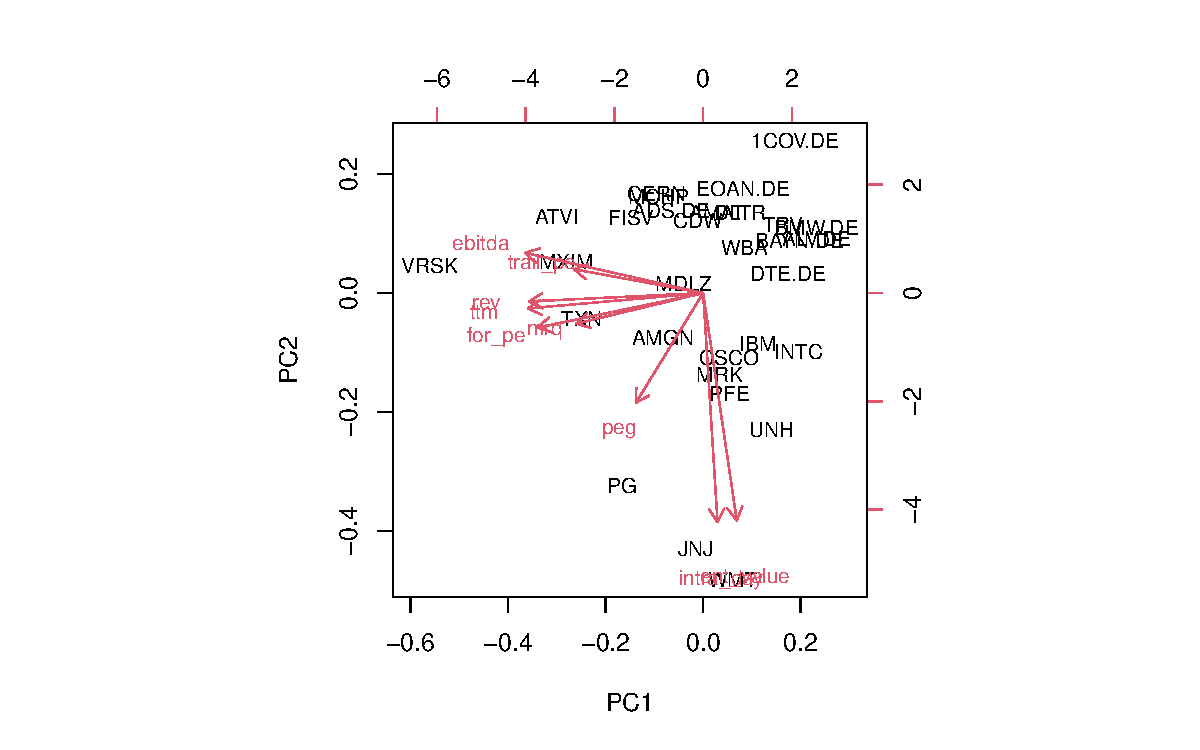
\includegraphics{ass2_files/figure-latex/bi-dis-1.pdf}
\caption{\label{fig:bi-dis}Distance Biplot of PCA of stocks' value}
\end{figure}

Distance biplot \ref{fig:bi-dis} indicates that \textbf{Johnson \& Johnson (JNJ)} and \textbf{Walmart (WMT)} have a high value in PC1, and \textbf{Activision Blizzard (ATVI)}, \textbf{Texas Instruments Incorporated (TXN)}, \textbf{Maxim Integrated Products (MXIM)} are higher in PC2.

Furthermore, we notice that \textbf{Verisk analytics (VRSK)} is a potential outlier for the PC1, \textbf{JNJ}, and \textbf{WMT} are potential outliers for PC2. The reason is based on the characteristic of these firms. Being a data-analytics and risk-assessment firm, \textbf{VRSK} provides the consulting service instead of the goods selling. Therefore, as for the financial sector, they profit generating will not directly lead to the increasing firm size. \textbf{JNJ} and \textbf{WMT} perform oppositely since they are operating as the multinational company. The continuously increasing market share will keep their profit at a high level.

\begin{table}

\caption{\label{tab:lim-1}Summary table of PCA for value analysis of stocks}
\centering
\begin{tabular}[t]{>{\raggedright\arraybackslash}p{70px}|r|r|r|r|r|r|r|r|r}
\hline
  & PC1 & PC2 & PC3 & PC4 & PC5 & PC6 & PC7 & PC8 & PC9\\
\hline
Standard deviation & 2.0468 & 1.4658 & 0.9319 & 0.9005 & 0.7316 & 0.5625 & 0.3081 & 0.1727 & 0.0784\\
\hline
Proportion of Variance & 0.4655 & 0.2387 & 0.0965 & 0.0901 & 0.0595 & 0.0352 & 0.0106 & 0.0033 & 0.0007\\
\hline
Cumulative Proportion & 0.4655 & 0.7042 & 0.8007 & 0.8908 & 0.9503 & 0.9855 & 0.9960 & 0.9993 & 1.0000\\
\hline
\end{tabular}
\end{table}

\begin{figure}
\centering
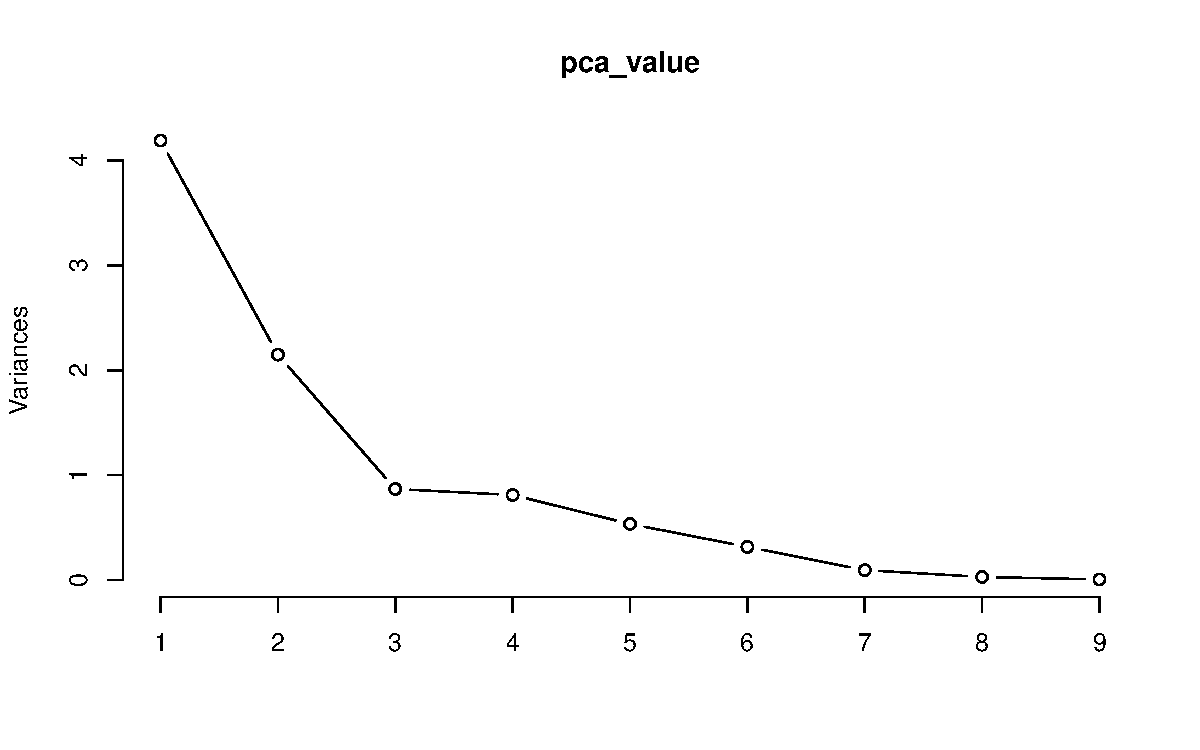
\includegraphics{ass2_files/figure-latex/lim-2-1.pdf}
\caption{\label{fig:lim-2}Screeplot of PCs in PCA for value analysis of stocks}
\end{figure}

The limitation of the value analysis also exists.

\begin{itemize}
\tightlist
\item
  After we filter out the outliers, the number of variables we put into use is 30 out of 147 and only 70.42\% of the overall variation could be explained by the first two principles (Table \ref{tab:lim-1}). The really small space size is not representative and also would not accurate enough to explain the whole stock market condition.
\item
  Screeplot (Figure \ref{fig:lim-2}) suggests the best PC selection is 3 which made the biplot 2 selection inadequate.
\end{itemize}

Therefore, we need to consider an alternative approach to make sure of the accuracy of our suggestion.

\hypertarget{risk-analysis}{%
\subsubsection{Risk Analysis}\label{risk-analysis}}

This part will provide a discussion about the potential risk of each stock based on the ESG risk score. We will compare the total risk score with the sum of the ESG scores to make sure the consistency of our data. Filtering out the inconsistent value would improve the accuracy of our results.

Table \ref{tab:pca-risk-summary} that PC1 and PC2 have explained almost 86\% of the total variation of 4 variables. Besides, Figure \ref{fig:pca-risk-screeplot} also suggests that the principal component of one and two should be selected because they all with a variance greater than 1 according to the Kaiser's Rule.

\begin{table}

\caption{\label{tab:pca-risk-summary}Summary table of PCA for risks analysis of stocks}
\centering
\begin{tabular}[t]{l|r|r|r|r}
\hline
  & PC1 & PC2 & PC3 & PC4\\
\hline
Standard deviation & 1.3946 & 1.2190 & 0.7544 & 0\\
\hline
Proportion of Variance & 0.4862 & 0.3715 & 0.1423 & 0\\
\hline
Cumulative Proportion & 0.4862 & 0.8577 & 1.0000 & 1\\
\hline
\end{tabular}
\end{table}

\begin{figure}
\centering
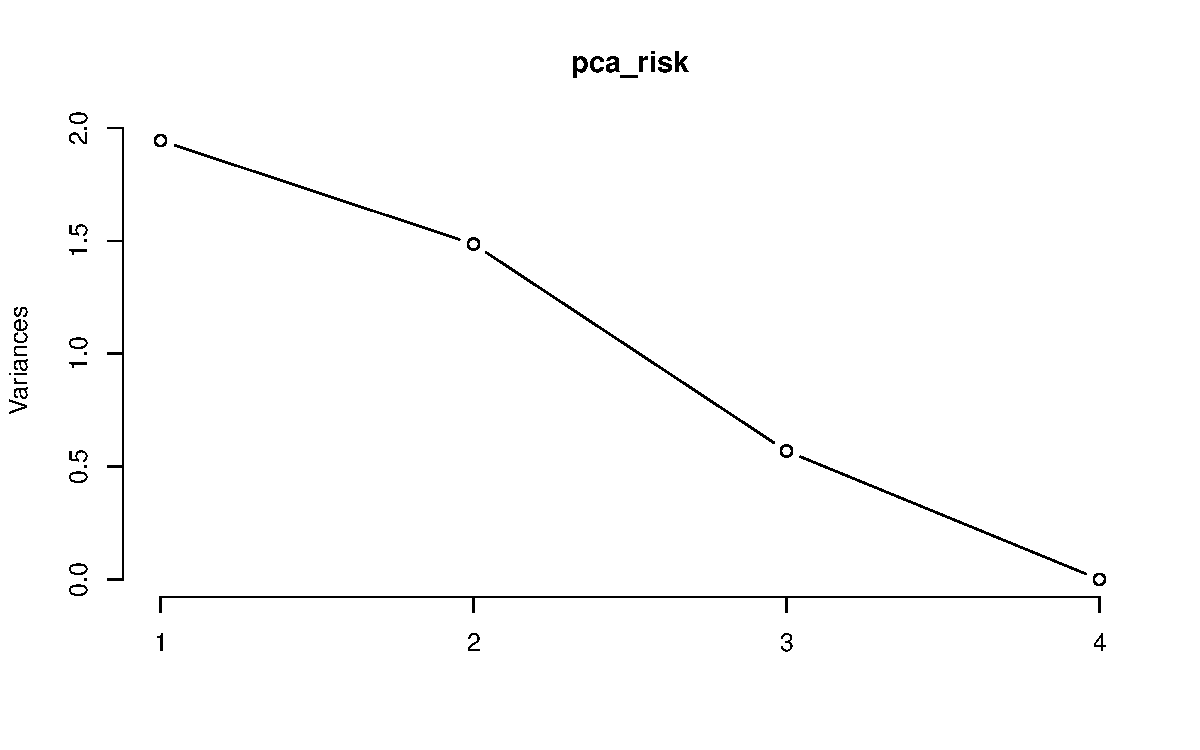
\includegraphics{ass2_files/figure-latex/pca-risk-screeplot-1.pdf}
\caption{\label{fig:pca-risk-screeplot}Screeplot of PCs in PCA for risk analysis of stocks}
\end{figure}

Figure \ref{fig:pca-risk-distance} shows the distance among each stock in the dataset and implies the similarity between stocks. The stocks of \textbf{VRSK} and \textbf{UnitedHealth Group Incorporated (UNH)} may be the same because they seem perfectly superimpose. Besides, \textbf{Allianz SE (ALV.DE)} and \textbf{Dollar Tree, Inc.~(DLTR)}, as well as \textbf{Cerner Corporation (CERN)} and \textbf{Fiserv, Inc.~(FISV)} might be similar, since they are close to each other. While the far distance between \textbf{VRSK} and \textbf{Microchip Technology Incorporated (MCHP)}, or \textbf{CDW Corporation (CDW)} and \textbf{Pfizer Inc.~(PFE)} indicate their different risk performance. To further analyzing the correlation between each stock, a correlation biplot is required.

\begin{figure}
\centering
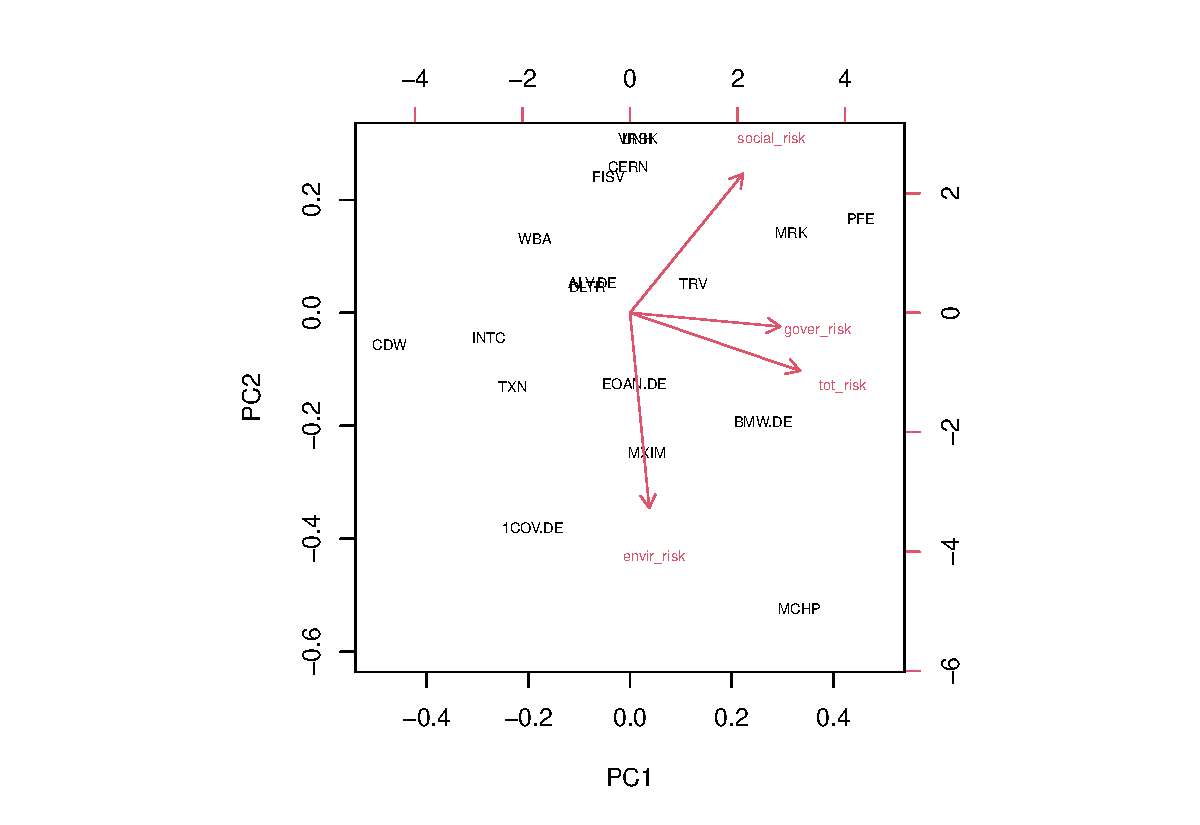
\includegraphics{ass2_files/figure-latex/pca-risk-distance-1.pdf}
\caption{\label{fig:pca-risk-distance}Distance biplot of PCA of stocks' risk}
\end{figure}

According to Figure \ref{fig:pca-risk-correlation} the correlation biplot \textbf{VRSK}, \textbf{UNH}, \textbf{CERN}, and \textbf{FISV} have the high values of social risk score, which indicate that these four stocks might perform better than the others in the social challenges. While they might not good at dealing with the risk from the environment since the social risk score and environmental risk score are approximately negative correlated. In contrast, \textbf{Covestro AG (1COV.DE)} and \textbf{MCHP} have the strongest abilities to face environmental challenges. Meanwhile, \textbf{MCHP} also has the highest score of governance risk, which indicates good performance in anticipating governance challenges. \textbf{PFE}, \textbf{Bayerische Motoren Werke AG (BMW.DE)}, and \textbf{Merck \& Co., Inc.~(MRK)} also perform well. While the projected positions of these three stocks along the axis of governance risk score are gradually decreasing, the approximate actual values of stock performance might gradually decline.

In general, based on the total ESG risk score, \textbf{MCHP} and \textbf{BMW.DE} have the best overall performance compared with other stocks, which indicate that their strategy in risk management is quite effective. Therefore, even if some external challenges occur, they will not have any significant fluctuations. In contrast, \textbf{CDW} has a weak overall risk performance for the low value in total risk score which indicates that the \textbf{CDW} stock price will not be stable when facing the risk.

\begin{figure}
\centering
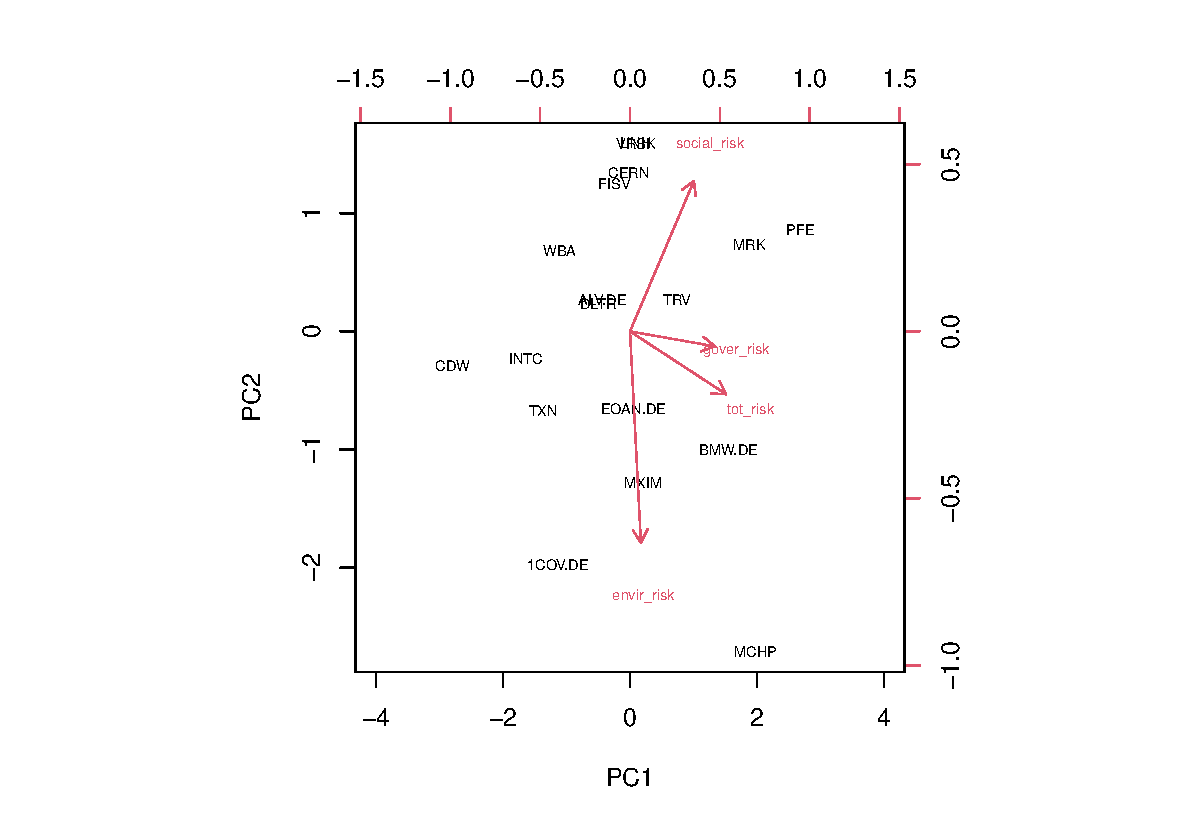
\includegraphics{ass2_files/figure-latex/pca-risk-correlation-1.pdf}
\caption{\label{fig:pca-risk-correlation}Correlation Biplot of PCA of stocks' risk}
\end{figure}

\hypertarget{cluster-analysis}{%
\subsection{Cluster Analysis}\label{cluster-analysis}}

Using the hierarchical clustering analysis with the agglomerative method, it is a bottom-up approach. We first select the data set that is consistent with the value data by equivalent stocks symbol. After standardised the data for the numeric variables, the Euclidian distance applied to find the distance between all pairs of observations. We employ Ward's methodology to sort the clusters. And the resulting clusters are shown in the dendrogram to display the sequences of merges or splits. Figure \ref{fig:ward} claims that two and four clusters of solutions are not stable. Hence, the three cluster solution is stable which is shown in \ref{fig:ward-3}.

\begin{figure}
\centering
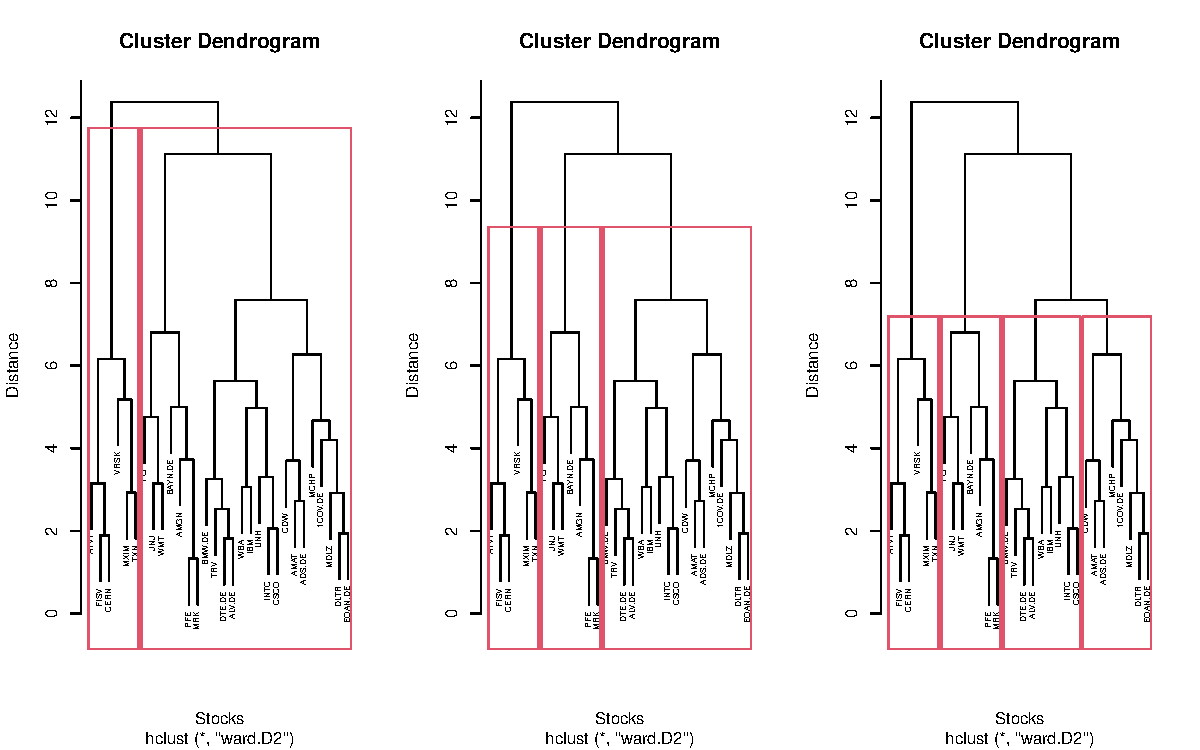
\includegraphics{ass2_files/figure-latex/ward-1.pdf}
\caption{\label{fig:ward}Choosing clusters}
\end{figure}

\begin{figure}
\centering
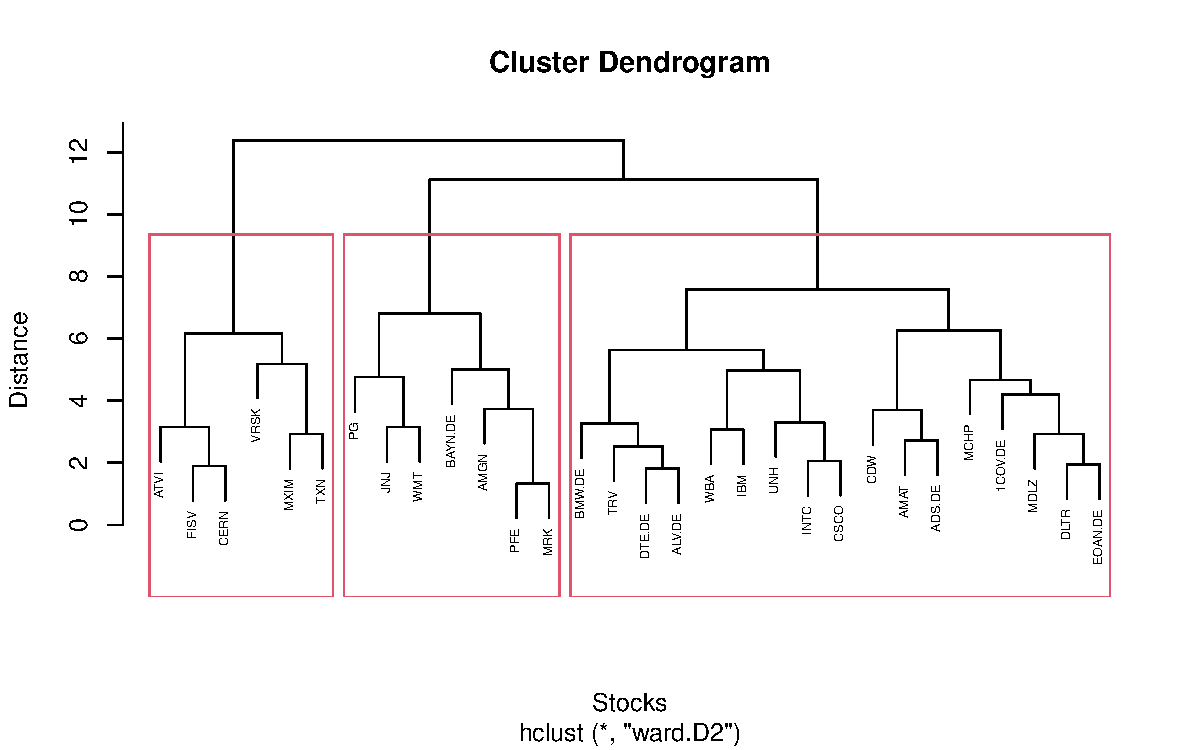
\includegraphics{ass2_files/figure-latex/ward-3-1.pdf}
\caption{\label{fig:ward-3}Dendogram using Ward methodology and taking Euclidian distances}
\end{figure}

From the dendrogram, there are three different clusters. These three clusters are shown in Table \ref{tab:memb-w}, Table \ref{tab:memb-two}, and Table \ref{tab:memb-three}, respectively.

\begin{table}

\caption{\label{tab:memb-w}The stocks of the first cluster}
\centering
\begin{tabular}[t]{l}
\hline
stock\\
\hline
Verisk Analytics, Inc.\\
\hline
Activision Blizzard, Inc.\\
\hline
Fiserv, Inc.\\
\hline
Maxim Integrated Products, Inc.\\
\hline
Texas Instruments Incorporated\\
\hline
Cerner Corporation\\
\hline
\end{tabular}
\end{table}

\begin{table}

\caption{\label{tab:memb-two}The stocks of the second cluster}
\centering
\begin{tabular}[t]{l}
\hline
stock\\
\hline
Amgen Inc.\\
\hline
Johnson \& Johnson\\
\hline
Pfizer Inc.\\
\hline
Walmart Inc.\\
\hline
Merck \& Co., Inc.\\
\hline
Bayer Aktiengesellschaft\\
\hline
The Procter \& Gamble Company\\
\hline
\end{tabular}
\end{table}

\begin{table}

\caption{\label{tab:memb-three}The stocks of the third cluster}
\centering
\begin{tabular}[t]{l}
\hline
stock\\
\hline
CDW Corporation\\
\hline
Microchip Technology Incorporated\\
\hline
Dollar Tree, Inc.\\
\hline
Mondelez International, Inc.\\
\hline
Applied Materials, Inc.\\
\hline
Intel Corporation\\
\hline
UnitedHealth Group Incorporated\\
\hline
Cisco Systems, Inc.\\
\hline
The Travelers Companies, Inc.\\
\hline
Walgreens Boots Alliance, Inc.\\
\hline
International Business Machines Corporation\\
\hline
E.ON SE\\
\hline
Deutsche Telekom AG\\
\hline
adidas AG\\
\hline
Bayerische Motoren Werke AG\\
\hline
Allianz SE\\
\hline
Covestro AG\\
\hline
\end{tabular}
\end{table}

\clearpage

\hypertarget{conclusions}{%
\section{Conclusions}\label{conclusions}}

According to our general evaluation of the Yahoo Finance market, we could say that \textbf{JNJ} and \textbf{WMT} perform better in company evaluation while \textbf{ATVI}, \textbf{TXN}, and \textbf{MXIM} are better in price and earning. \textbf{VRSK}, \textbf{JNJ} and \textbf{WMT} could be considered as the special cases since they outperform in their area. What ESG risk analysis provides us is that \textbf{MCHP} and \textbf{BMW.DE} have a great performance in overall anti-risk, some other companies perform better in a specific risk score. For instance, \textbf{UNH}, \textbf{CERN}, and \textbf{FISV} perform well in anti-social risk, but they are not resilient enough when meeting the challenges from environmental risk compared with \textbf{1COV.DE} and \textbf{MCHP}. And our investment suggestions are listed below:

\begin{itemize}
\tightlist
\item
  Fully consider the characteristics of the firm and consider the factors which might dominate the stock value.
\item
  Both internal and external risks would on the value of stocks and will generate the fluctuation of prices in the stock market as well.
\item
  Investors need to make the investment decision based on their risk tolerance and well balance differences in the risk-control of each company.
\item
  Companies need to improve the ability of self-resilience and anti-risks so than enhance the performance when facing different types of risks.
\end{itemize}

\clearpage

\hypertarget{acknowledgement}{%
\section{Acknowledgement}\label{acknowledgement}}

The data could be downloaded from \href{https://au.finance.yahoo.com/}{Yahoo Finance}. Meanwhile, the report uses the template called \textbf{Monash Consulting Report} which could use by downloading the package called \href{https://github.com/robjhyndman/MonashEBSTemplates}{MonashEBSTemplates}. In addition, the programming language used to analyse the stocks is R (4.0.2) (R Core Team, 2020).

Following packages has been included in our Rmd file:

\begin{itemize}
\tightlist
\item
  package dplyr (1.0.1) (Wickham et al., 2020),
\item
  package ggplot2 (3.3.2) (Wickham, 2016),
\item
  package tidyverse (1.3.0) (Wickham et al., 2019),
\item
  package mclust (5.4.6) (Scrucca et al., 2016),
\item
  package visdat (0.5.3) (Tierney, 2017),
\item
  package gridExtra (2.3) (Auguie, 2017),
\item
  package kableExtra (1.1.0) (Zhu, 2019),
\item
  package tibble (3.0.3) (Müller \& Wickham, 2020).
\end{itemize}

\clearpage

\hypertarget{references}{%
\section{References}\label{references}}

Auguie, B. (2017). Gridextra: Miscellaneous functions for ``grid'' graphics {[}R package version 2.3{]}.
\url{https://CRAN.R-project.org/package=gridExtra}

Müller, K, \& Wickham, H. (2020). Tibble: Simple data frames {[}R package version 3.0.3{]}. \url{https://CRAN.R-project.org/package=tibble}

R Core Team. (2020). R: A language and environment for statistical computing. R Foundation for Statistical Computing. Vienna, Austria. \url{https://www.R-project.org/}

Scrucca, L, Fop, M, Murphy, TB, \& Raftery, AE. (2016). mclust 5: Clustering, classification and density
estimation using Gaussian finite mixture models. The R Journal, 8(1), 289--317.

Tierney, N. (2017). Visdat: Visualising whole data frames. JOSS, 2(16), 355.

Wickham, H. (2016). Ggplot2: Elegant graphics for data analysis. Springer-Verlag New York. \url{https://ggplot2.tidyverse.org}

Wickham, H, Averick, M, Bryan, J, Chang, W, McGowan, LD, François, R, Grolemund, G, Hayes, A,
Henry, L, Hester, J, Kuhn, M, Pedersen, TL, Miller, E, Bache, SM, Müller, K, Ooms, J, Robinson,
D, Seidel, DP, Spinu, V, \ldots{} Yutani, H. (2019). Welcome to the tidyverse. Journal of Open
Source Software, 4(43), 1686.

Wickham, H, François, R, Henry, L, \& Müller, K. (2020). Dplyr: A grammar of data manipulation {[}R
package version 1.0.1{]}. \url{https://CRAN.R-project.org/package=dplyr}

Zhu, H. (2019). Kableextra: Construct complex table with 'kable' and pipe syntax {[}R package version
1.1.0{]}. \url{https://CRAN.R-project.org/package=kableExtra}

\clearpage

\appendix

\hypertarget{appendix}{%
\section{Appendix}\label{appendix}}

\hypertarget{ends-with-emphasis}{%
\subsection{Ends with Emphasis}\label{ends-with-emphasis}}

At the end of our report, it is necessary to emphasis that due to the small sample space and the incomplete eigenvalue selection, our result might not be representative and the biplot could not fully state the overall situation. Even though, in our case, the biplot is suitable for risk analysis. We still could not deny the fact that in general, the small sample size would lead to the bias in output. Therefore, our report uses cluster analysis as an alternative approach. The agglomerative method indicates that a stable solution is three clusters. And here we would show complete linkage method (Figure \ref{fig:complete}), average linkage (Figure \ref{fig:average}) and centroid method (Figure \ref{fig:centroid}). In order to check the robustness, we compute the adjusted rand index using \texttt{adjustedRandIndex} function. Table \ref{tab:adjusted-index} indicates that the complete linkage method has a relatively high level of agreement with Ward's method.

\begin{figure}
\centering
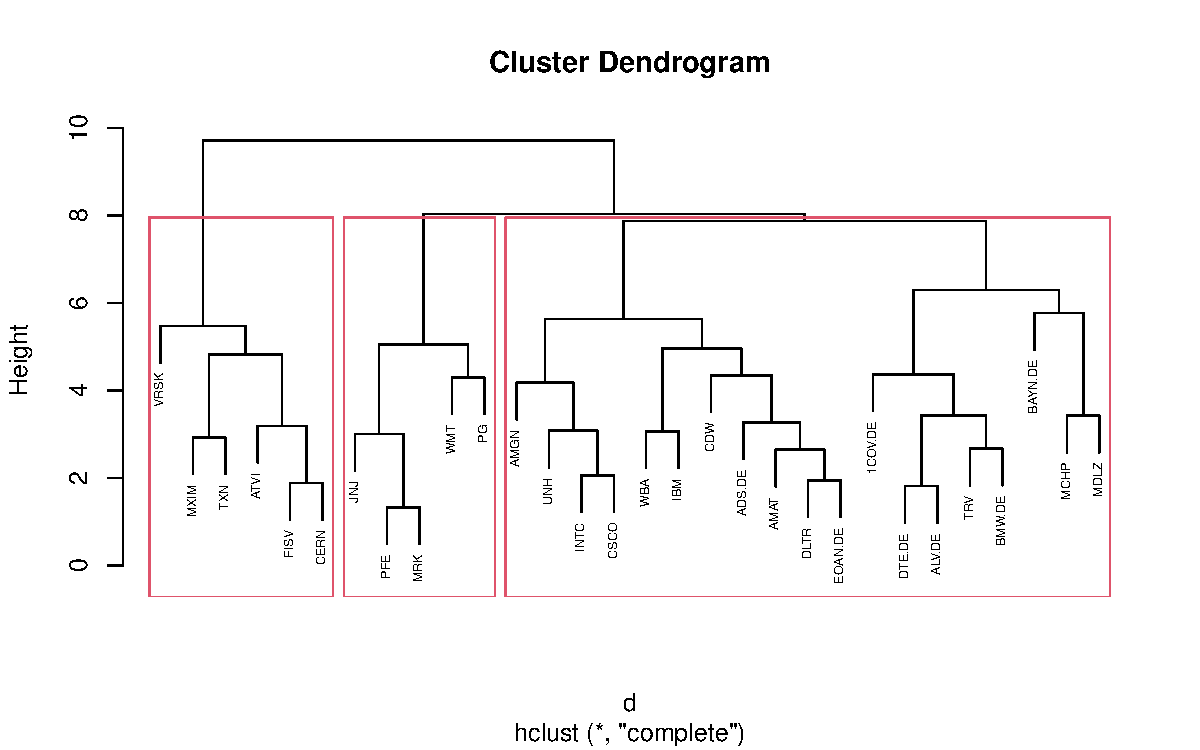
\includegraphics{ass2_files/figure-latex/complete-1.pdf}
\caption{\label{fig:complete}Cluster dendrogram of complete linkage method}
\end{figure}

\begin{figure}
\centering
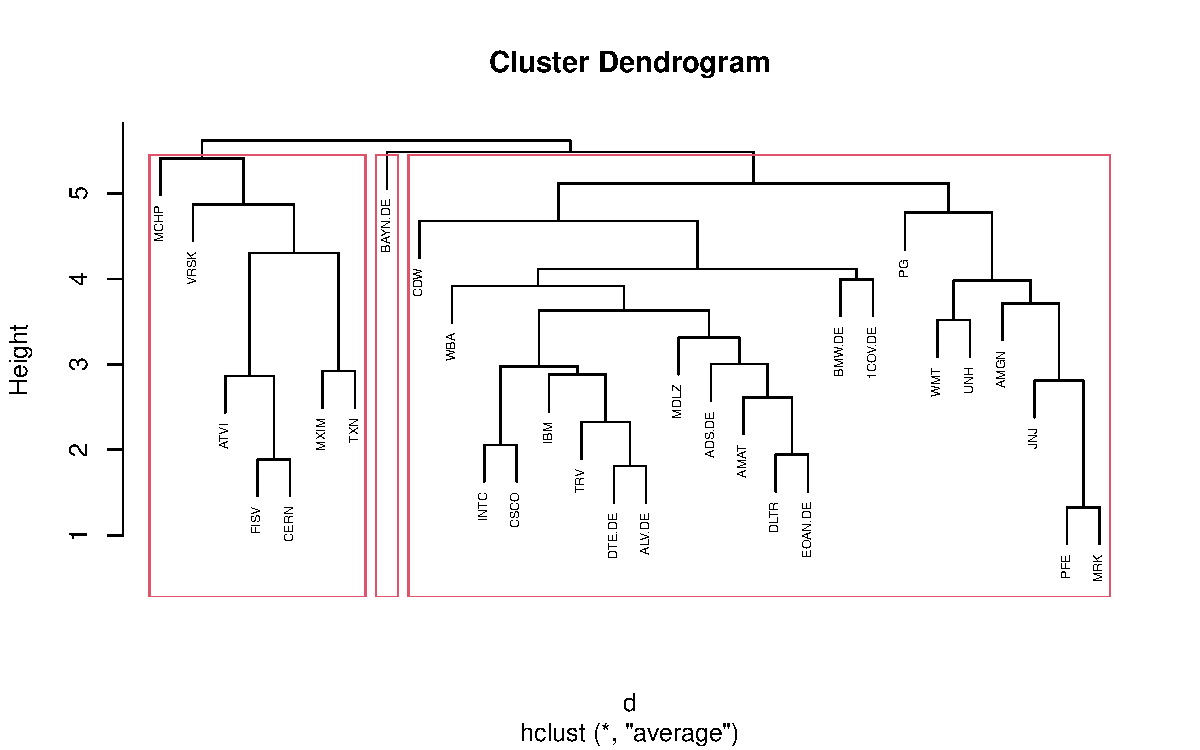
\includegraphics{ass2_files/figure-latex/average-1.pdf}
\caption{\label{fig:average}Cluster dendrogram of average linkage method}
\end{figure}

\begin{figure}
\centering
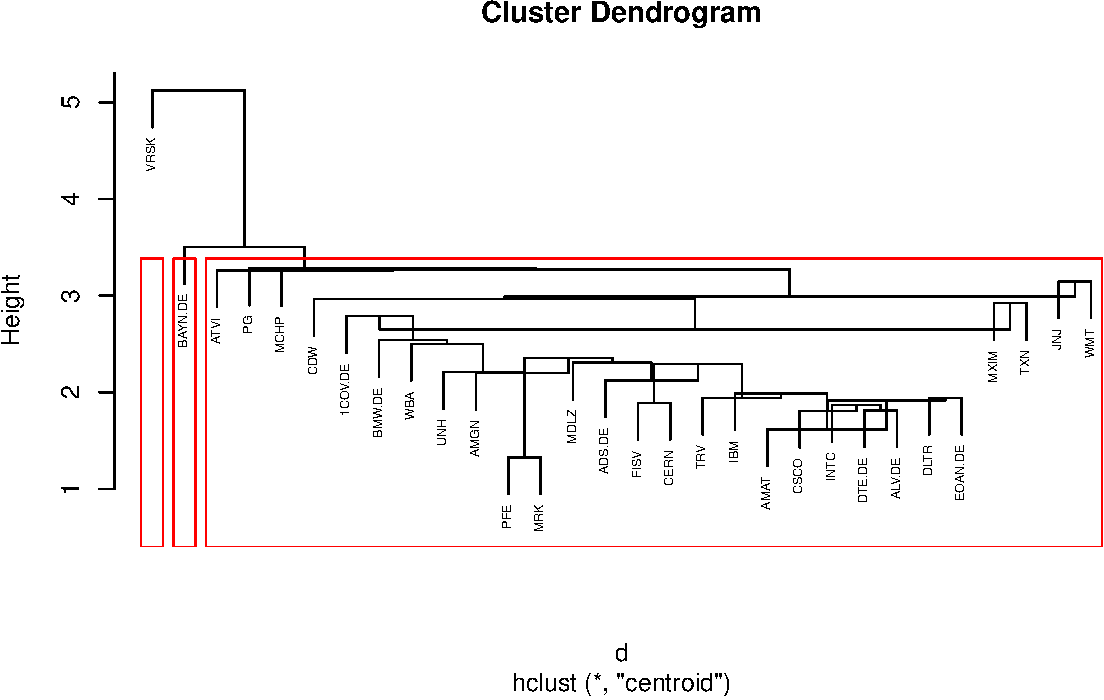
\includegraphics{ass2_files/figure-latex/centroid-1.pdf}
\caption{\label{fig:centroid}Cluster dendrogram of centroid method}
\end{figure}

\begin{table}

\caption{\label{tab:adjusted-index}The adjusted rand index of the three clustering methods}
\centering
\begin{tabular}[t]{l|r}
\hline
  & adjusted rand index\\
\hline
complete linkage method & 0.7934295\\
\hline
average linkage method & 0.4481954\\
\hline
centroid method & 0.0919079\\
\hline
\end{tabular}
\end{table}

\printbibliography

\end{document}

